\RequirePackage{kvoptions-patch}
\documentclass[titre=Stastistiques, classe=Troisième]{jeanmonnet}

\newcounter{countvaleurs}

\setsepchar{;}
\readlist\valeurs{3;1;6;2;2;1;4;5;1;4;6;3;2;3;3;5;5;6;1;2;6;1;2;1;4;3;3;4;3;6}
\newcommand{\displayvaleurs}{
	\setcounter{countvaleurs}{1}
	\multido{}{\valeurslen}{
		\valeurs[\arabic{countvaleurs}] %
		\stepcounter{countvaleurs}
	}
}


\begin{document}
\chapter{\titre}

\section{Statistiques discrètes}
\subsection{Un peu de vocabulaire}

On se place dans la situation suivante :

\begin{quote}
Dans une classe, les élèves ont lancé un dé cubique dont les faces sont numérotées de $1$ à $6$ et ont noté le résultat. Les voici :

\displayvaleurs	
\end{quote}

\begin{definition}{Vocabulaire}{}
	Les résultats précédents constituent un \emph{relevé statistique}.
	\begin{itemize}
		\item La \emph{population étudiée} est l'ensemble des élèves de cette classe.
		\item Le \emph{caractère étudié} est le résultat d'un lancer de dé.
		\item Les \emph{données du caractère} sont les $20$ résultats obtenus.
		\item Les \emph{valeurs du caractère} sont les valeurs prises par celui-ci, soit $1,2,3,4,5$ ou $6$.
	\end{itemize}
\end{definition}

\begin{definition}{Effectifs}{}
	L'\textbf{effectif} d'une valeur est le nombre de fois où cette valeur apparaît.
	
	L'\textbf{effectif total} est la somme des effectifs : c'est le nombre total de valeurs.
\end{definition}

\begin{exemple}{Calcul de l'effectif total de la série exemple}{}
Le calcul de l'effectif total est alors :
\[ 6+5+7+4+3+5 = 30\]
\end{exemple}

\begin{exemple}{Représentation de la série exemple dans un tableau}{}
L'ensemble des données précédentes peut être représenté dans un \emph{tableau des effectifs}.

\begin{figure}[H]
\begin{center}
	\begin{tabular}{|*{7}{c|}}
		\hline
		Face & 1 & 2 & 3 & 4 & 5 & 6 \\
		\hline
		Effectifs & 6&5&7&4&3&5\\
		\hline
	\end{tabular}
\end{center}
\caption{Tableau des effectifs}
\end{figure}
\end{exemple}

\begin{definition}{Effectif cumulé croissant}{}
	L'effectif cumulé croissant d'une valeur est la somme de l'effectif de cette valeur et de toutes les valeurs inférieures à cette dernière.	
\end{definition}


\begin{figure}[H]
\begin{center}
	\begin{tabular}{|*{7}{c|}}
		\hline
		Face & 1 & 2 & 3 & 4 & 5 & 6 \\
		\hline
		Effectifs & 6&5&7&4&3&5\\
		\hline
		Effectifs cumulés& 6 & 6+5 & 6+5+7 & 6+5+7+4 & 6+5+7+4+3 & 6+5+7+4+3+5\\
		croissants & = 6 & = 11 & = 18 & = 22 & = 25 & = 30\\
		\hline
	\end{tabular}
\end{center}
\caption{Tableau des effectifs cumulés croissants de la série exemple}
\end{figure}	

\subsection{Fréquences}

\begin{definition}{Fréquence}{}
	La \textbf{fréquence} d'une valeur est le quotient de l'effectif de la valeur par l'effectif total. Cette valeur est comprise entre $0$ et $1$. Le résultat peut aussi être donné en pourcentage (compris entre $1$ et $100$).
	
	\[\mbox{fréquence valeur} = \dfrac{\mbox{effectif de la valeur}}{\mbox{effectif total}}\]
	
	\begin{align*}
	\mbox{fréquence valeur pourcentage}
		& = \dfrac{\mbox{effectif de la valeur}}{\mbox{effectif total}} \times 100\\
		& = \mbox{fréquence valeur} \times 100
	\end{align*}
\end{definition}

\begin{proof}
	On considère un relevé statistique d'effectif total $E$. On note $v_0$ l'une des valeurs de ce relevé et $e_0$ l'effectif associé.
	Alors :
	\[\mbox{fréquence }_{v_0} = \dfrac{e_0}{E}\]
	Or $E$ est la somme des effectifs et ces derniers sont tous positifs, on en déduit l'inégalité suivante :
	\[0\leq e_0\leq E\]
	Ce qui prouve\footnote{Pour être exact, il faudrait remarquer ici que $E$ est positif.} que 
	\[0 = \dfrac{0}{E} \leq \dfrac{e_0}{E} \leq\dfrac{E}{E} = 1\]
	
	L'inégalité des fréquences en pourcentage est alors un corollaire.
\end{proof}

\begin{figure}[H]
	\begin{center}
	\renewcommand{\arraystretch}{3}
		\begin{tabular} {|p{4cm}|*{6}{p{1.5cm}|}}
		\hline
		Face & 1 & 2 & 3 & 4 & 5 & 6 \\
		\hline
		Fréquence (exacte) & $\dfrac{6}{30}$&$\dfrac{5}{30}$&$\dfrac{7}{30}$&$\dfrac{4}{30}$&$\dfrac{3}{30}$&$\dfrac{5}{30}$\\
		\hline
		Fréquence ($\simeq$) & $0.2$&$0.17$&$0.23$&$0.13$&$0.1$&$0.17$\\
		\hline
		Fréquence ($\%$) & $20.0$&$16.7$&$23.3$&$13.3$&$10.0$&$16.7$\\
		\hline
		\end{tabular}
	\end{center}
	\caption{Tableau des fréquences de la série exemple}
\end{figure}

\subsection{Représentation graphique}

Pour représenter un relevé statistique dans le cas discret, on réalise un \emph{digramme en bâtons}.

\begin{definition}{Diagramme en bâtons}{}
	Un diagramme en bâtons est un diagramme composé :
	\begin{itemize}
	\item en abscisses, des différentes valeurs ;
	\item en ordonnées, de l'effectif ou de la fréquence de chaque valeur.
	\end{itemize}
\end{definition}

\begin{figure}[H]
\centering
	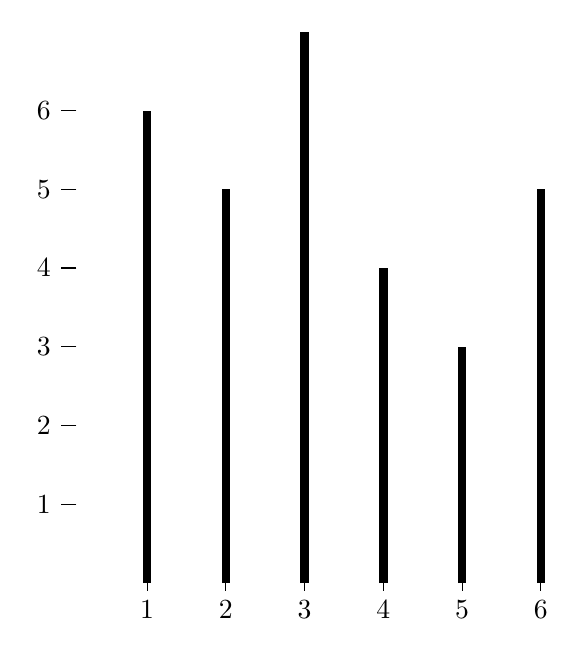
\begin{tikzpicture}
		\repere{0}{7}{0}{7}{1}
%		\draw[color = gray!40] (0,0) grid (7,7);
		\foreach \k in {1,2,...,6}{
			\draw (\k,0.1) -- (\k,-0.1) node[below]{$\k$};
			\draw (0.1,\k) -- (-0.1,\k) node[left]{$\k$};
		}
		\foreach \k/\i in {1/6,2/5,3/7,4/4,5/3,6/5}{
			\draw[line width=3pt] (\k,0) -- (\k,\i);
		}
		%
		% Valeurs
		%
	\end{tikzpicture}
	\caption{Représentation par un diagramme en bâton de la série exemple}
\end{figure}

\subsection{Indicateurs et critère}
\subsubsection{Moyenne}

\begin{definition}{Moyenne}{}
	La moyenne d'une série est la valeur que devraient avoir toutes les valeurs d'une série de même effectif pour obtenir la même moyenne.
\end{definition}

\begin{propriete}{Calcul de la moyenne}{}
	Soit une série statistique dont les valeurs sont $v_1, \dots, v_n$ et les effectifs associés $e_1, \dots, e_n$.
	\begin{itemize}
		\item La \textbf{moyenne simple} de cette série est \emph{le quotient de la somme des valeurs par l'effectif total}.
		\begin{align*}
			\mbox{moyenne simple}
			& = \dfrac{\mbox{somme des valeurs}}{\mbox{effectif total}}
		\end{align*}
		\item La \textbf{moyenne pondérée} de cette série est \emph{le quotient des produits des valeurs par leur effectif par l'effectif total}.
		\begin{align*}	
			\mbox{moyenne pondérée}
			& = \dfrac{\mbox{somme des valeur fois effectif}}{\mbox{effectif total}}\\
			& = \dfrac{v_1\times e_1 + \cdots + v_n\times e_n}{e_1 + \cdots + e_n}
		\end{align*}
	\end{itemize}
\end{propriete}

\begin{exemple}{Moyenne simple de la série}{}
	On réalise le calcul de la moyenne simple $m$.
	\begin{align*}
		m
		& = (3+1+6+2+2+1+4+5+1+4+6+3+2+3+3\\
		&\qquad\dfrac{+5+5+6+1+2+6+1+2+1+4+3+3+4+3+6)}{30}\\
		& \simeq 3.27
	\end{align*}
	La moyenne $m$ est environ $3,27$.
\end{exemple}

\begin{exemple}{Moyenne pondérée de la série}{}
	On réalise le calcul de la moyenne pondérée $m'$.
	\begin{align*}
		m' 
		& = \dfrac{1\times6 +2\times5 +3\times7 +4\times4 +5\times3 +6\times5 }{30}\\
		& \simeq 3.27
	\end{align*}
\end{exemple}

On remarque que les deux calculs donnent le même résultat. On pourra donc choisir la méthode de son choix pour réaliser le calcul d'une moyenne.

\subsubsection{Etendue}

\begin{definition}{Etendue}{}
	L'étendue d'une série statistique est l'écart entre la plus grande et la plus petite valeur d'une série.
\end{definition}

\begin{propriete}{Calcul de l'étendue}{}
	L'étendue d'une série est obtenue en retranchant la plus petite valeur de la série à la plus grande valeur de la série.
\end{propriete}

\begin{exemple}{Etendue de la série exemple}{}
	La plus grande valeur de la série est $6$ et la plus petite valeur est $1$.
	\[e = 6 - 1 = 5\]
	L'étendue de la série est donc $5$.
\end{exemple}

\subsubsection{Médiane}

\begin{definition}{Médiane}{}
	La médiane d'une série statistique est la valeur, prise par la série ou non, qui partage l'effectif ordonné en deux parties égales.
\end{definition}

En interprétation, on utilisera la phrase suivante :
\begin{quote}
	Au moins 50\% de l'effectif a une valeur inférieure à la médiane et au moins 50\% de l'effectif a une valeur supérieure à la médiane.
\end{quote}


\begin{propriete}{Calcul de la médiane}{}
	Il existe deux cas pratiques pour le calcul de la médiane.	\begin{description}
		\item[Cas impair] Si l'effectif total est impair, la médiane est la valeur centrale de la série ordonnée. Si l'effectif total est $2n+1$, alors la médiane est la $n+1$\ieme valeur.
		\item[Cas pair] Si l'effectif total est pair, la médiane est une valeur comprise entre les deux valeurs centrales de la série ordonnée. Si l'effectif total est $2n$, alors la médiane est n'importe quel nombre situé entre la $n\ieme$ et la $n+1\ieme$ valeurs.
	\end{description}
\end{propriete}

\begin{exemple}{Médiane de la série exemple}{}
	L'effectif total de cette série est pair : $30 = 2 \times 15$. On en déduit que la médiane est située entre la $15$\ieme et la $16$\ieme valeur de la série ordonnée.
	
	D'après le tableau des effectifs, en particulier les effectifs cumulés croissants, on remarque que ces deux valeurs valent $3$. 
	
	La médiane de la série est $3$.
	Ainsi au moins $50$\% des résultats de la série sont inférieurs à $3$ et au moins $50$\% des résultats de la série sont supérieurs à $3$.
\end{exemple}

\section{Statistiques continues}

%Les statistiques continues sont utilisées lorsque les valeurs ne peuvent plus être dénombrées facilement et peuvent prendre un nombre très grand de valeurs. On utilise alors de classe pour les regrouper. 


\begin{definition}{Classe}{}
	\renewcommand{\thefootnote}{\arabic{footnote}}
	Une classe\footnote{La notation utilisée ici est la notation standard qui permet aussi de définir la notion d'intervalle. En particulier, ici l'intervalle est \og fermé à gauche\fg{} et \og ouvert à droite\fg{}.} est toujours notée $[a;b[$. 
	\begin{itemize}
		\item $a$ est la plus petite valeur possible de la classe et peut être atteinte.
		\item $b$ est la plus grande valeur possible de la classe mais sans jamais l'atteindre.
	\end{itemize}
	L'amplitude d'une classe est la valeur $b-a$.
	
	\textbf{Attention :} pour plus de simplicité, on gardera toujours des classes de même amplitude.
\end{definition}

On considère dans cette section le cas suivant:
\begin{quote}
	Une enquête a permis de relever le prix d'un article dans 15 points de vente différents. On obtient la liste suivante :
	\[11,29 ; 12,30 ; 12,05; 11 ; 11,48 ; 10,85 ; 13,19 ; 10,70 ; 12,43 ; 12,06 ; 13,50 ; 11,82 ; 12 ; 12,55 ; 12,34\]
\end{quote}

On a alors les caractéristiques suivantes :
\begin{itemize}
	\item population étudiée : les 15 points de vente ;
	\item caractère étudié : le prix de l'article ;
	\item valeurs du caractère : les différents prix de la liste.
\end{itemize}

On peut alors regrouper ces données dans un tableau.

\begin{figure}[H]
	\centering
	\renewcommand{\arraystretch}{3}
	\begin{tabular}{|*{5}{c|}}
		\hline
		Prix & $[10,11[$&$[11,12[$&$[12,13[$&$[13,14[$\\
		\hline
		Effectifs & 2&4&7&2\\
		\hline
		Fréquence ($\simeq$) & $0.13$&$0.27$&$0.47$&$0.13$\\
		\hline
		Fréquence (exacte) & $\dfrac{2}{15}$&$\dfrac{4}{15}$&$\dfrac{7}{15}$&$\dfrac{2}{15}$\\
		\hline
	\end{tabular}
	\caption{Tableau dans le cas d'une série continue}
\end{figure}

La représentation dans un tel cas est un \emph{histogramme}

\begin{figure}[H]
\centering
	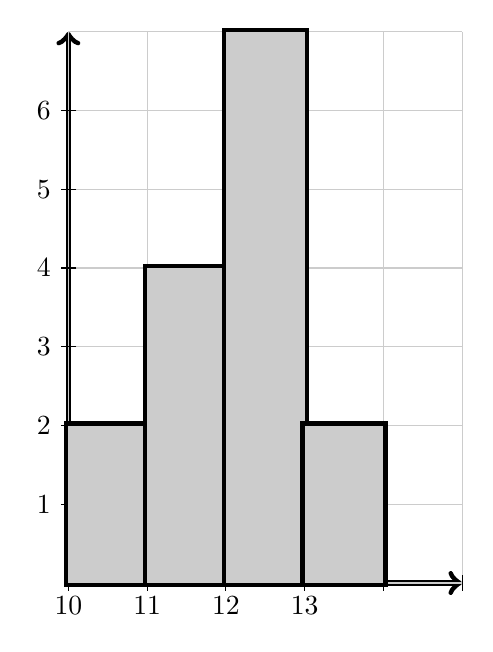
\begin{tikzpicture}
		\draw[->, line width=2pt](10,0) -- (15,0);
		\draw[->, line width=2pt](10,0) -- (10,7);
		\draw[color = gray!40] (10,0) grid (15,7);
%		\draw[color = gray!40] (0,0) grid (7,7);
		\foreach \k in {1,2,...,6}{
			\draw (9+\k,0.1) -- (9+\k,-0.1);
			\draw (10+0.1,\k) -- (10-0.1,\k)node[left]{$\k$};
		}
		\foreach \k/\i in {10/2,11/4,12/7,13/2}{
			\draw[line width=3pt] (\k,0)node[below]{$\k$} -- (\k,\i) -- (\k+1,\i) -- (\k+1,0)--cycle;
			\fill[color=gray!40] (\k,0) -- (\k,\i) -- (\k+1,\i) -- (\k+1,0)--cycle;
		}
		%
		% Valeurs
		%
	\end{tikzpicture}
	\caption{Représentation d'un relevé statistique par un diagramme en bâton}
\end{figure}

\section{Valeurs non numériques}

Dans le cas d'une étude statistique, il est possible que les valeurs ne soient pas numériques.

\begin{quote}
	Dans un groupe de 10 élèves, on liste les langues vivantes 1 pratiquées par chacun.

\bigskip

	Anglais - Anglais - Allemand - Espagnol - Anglais - Espagnol - Espagnol - Anglais - Anglais - Anglais
\end{quote}

La représentation d'une telle série peut se faire à l'aide d'un diagramme circulaire.

\begin{definition}{Diagramme circulaire}{}
	Un diagramme circulaire est un disque découpé en secteur. Chaque secteur a un angle (et donc une aire) proportionnel à l'effectif de la valeur représentée.
\end{definition}

\begin{minipage}{0.5\linewidth}
\begin{figure}[H]
\centering
\renewcommand{\arraystretch}{3}
	\begin{tabular}{|*{4}{c|}}
	\hline
	Langue & Anglais & 	Espagnol & Allemand \\
	\hline
	Effectif & 6 & 3 & 1 \\
	\hline
	Angle (calcul) & $\dfrac{6}{10}\times 360$ & $\dfrac{3}{10}\times 360$ & $\dfrac{1}{10}\times 360$ \\
	\hline
	Angle & $216$\degres & $108$\degres & $36$\degres\\
	\hline
	\end{tabular}
	\caption{Tableau des effectifs et calcul d'angles}
\end{figure}
\end{minipage}
\begin{minipage}{0.5\linewidth}
\begin{figure}[H]
	\centering
	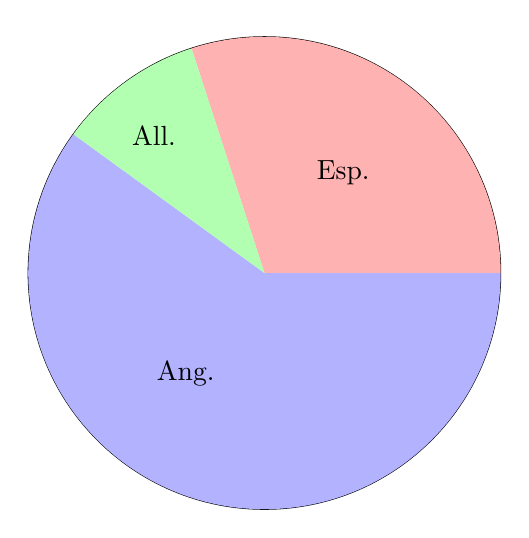
\begin{tikzpicture}
		\draw (0,0) circle (3cm);
		\fill[color = red!30] (0,0) -- (3,0) arc (0:108:3) -- (0,0);
		\fill[color = blue!30] (0,0) -- (3,0) arc (0:-216:3) -- (0,0);
		\fill[color = green!30] (0,0) -- (108:3) arc (108:144:3) -- (0,0);
		\draw (-1,1.5)node[above left]{All.};
		\draw (-1,-1)node[below]{Ang.};
		\draw (1,1)node[above]{Esp.};
		
	\end{tikzpicture}
	\caption{Diagramme circulaire}
\end{figure}
\end{minipage}
\end{document}